% version 1.00, date 10/10/16, auteur Kafui Atanley
Ce chapitre décrit les différents diagrammes d'intéraction.

\section{Fonctionnalité 8}
Ce paragraphe décrit le diagramme d'intéraction concernant la fonctionnalité 8 soit la géolocalisation. \\

La figure suivant (figure \ref{diagrammeInteraction1}) indique le déroulement de la consultation d'une entité possédant une adresse.
\begin{figure}[H]
	\centering
	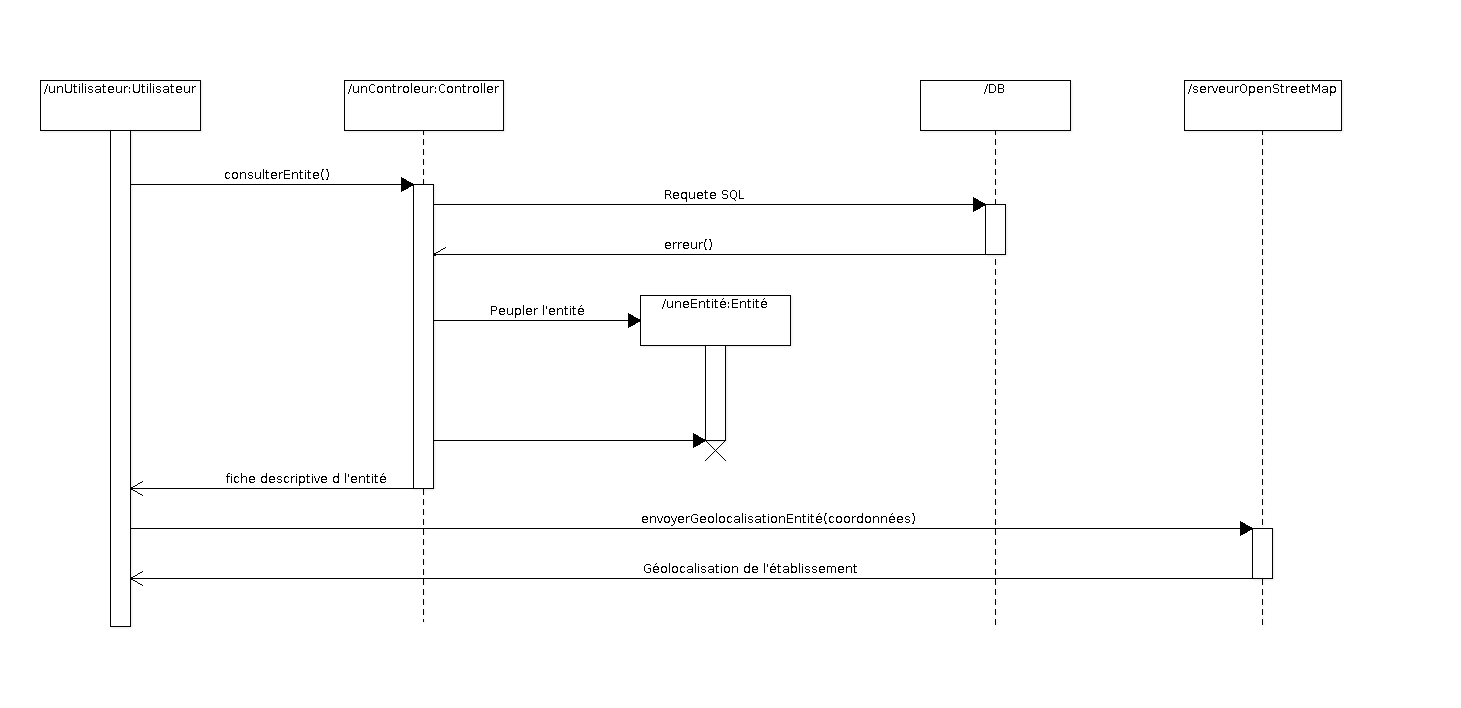
\includegraphics[scale=0.39]{images/diagrammesInteraction/01_diagrammeInteractionF8.png}
	\caption{Diagramme d'intéraction~: consultation d'une entité possédant une adresse}
	\label{diagrammeInteraction1}
\end{figure}

La figure suivante (figure \ref{diagrammeInteraction2}) indique le déroulement de la connexion et la déconnexion d'un bénévole.
%\begin{figure}[H]
%	\centering
%	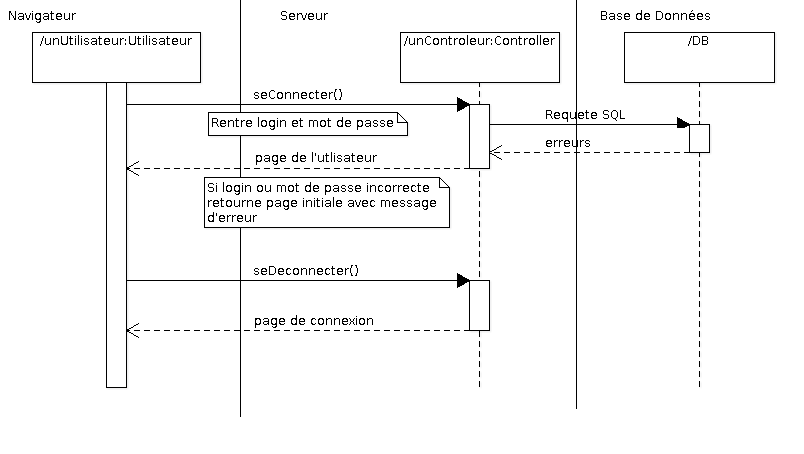
\includegraphics[scale=0.65]{images/diagrammesInteraction/02_diagrammeInteractionF1.png}
%	\caption{Diagramme d'intéraction~: Connection et déconnection d'un utilisateur}
%	\label{diagrammeInteraciton2}
%\end{figure}

\section{Fonctionnalité 9}
Ce paragraphe décrit le diagramme d'intéraction concernant la fonctionnalité 9 soit l'attribution de frimousse. \\

La figure suivante (figure \ref{diagrammeInteraction3}) indique le déroulement de la création, la modification et la suppression d'un établissement par un administrateur.
%\begin{figure}[H]
%	\centering
%	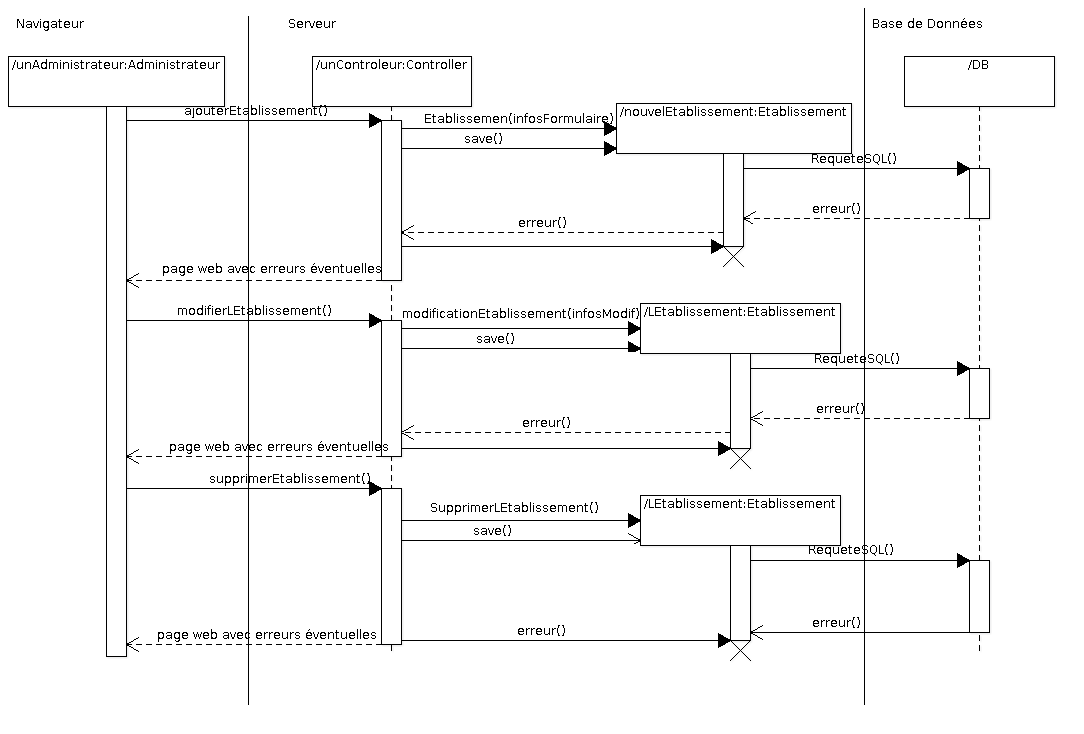
\includegraphics[scale=0.5]{images/diagrammesInteraction/03_diagrammeInteractionF2.png}
%	\caption{Diagramme d'intéraction~: Création, modification, suppression d'un établissement par un administrateur}
%	\label{diagrammeInteraction3}
%\end{figure}

\section{Fonctionnalité 10}
Ce paragraphe décrit le diagramme d'intéraction concernant la fonctionnalité 10 soit la gestion des ventes. \\

La figure suivante (figure \ref{diagrammeInteraction4}) indique le déroulement de l'envoi du formulaire de demande d'intervention aux établissements.
%\begin{figure}[H]
%	\centering
%	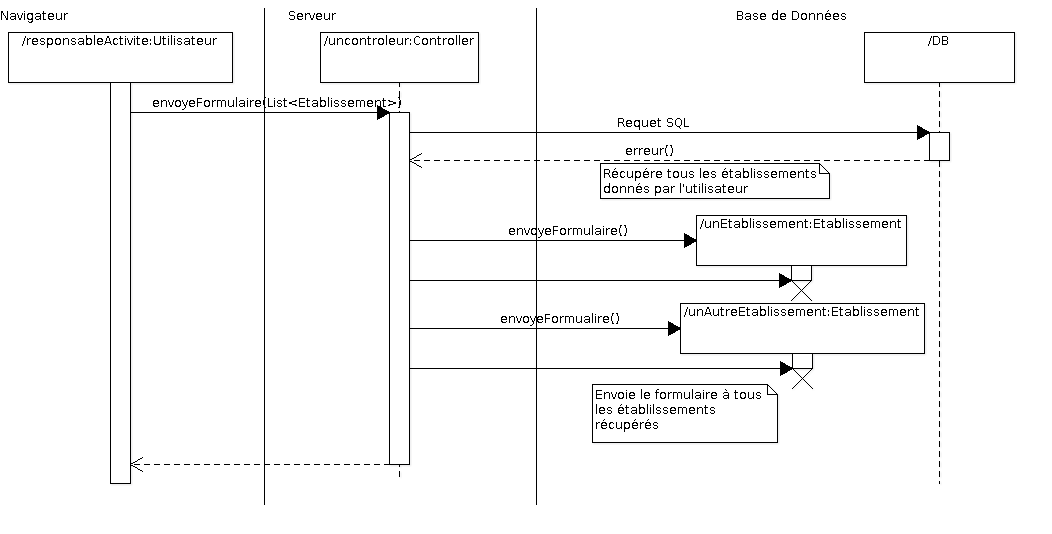
\includegraphics[scale=0.5]{images/diagrammesInteraction/04_diagrammeInteractionF3.png}
%	\caption{Diagramme d'intéraction~: Envoye du formulaire à un ensemble d'établissement}
%	\label{diagrammeInteraction4}
%\end{figure}



